\ifx\wholebook\relax\else
\input{../Common.tex}
\input{../macroes.tex}
\begin{document}
\fi


%ch:Evaluating
\chapter{Boolean and Boolean Expressions}\label{cha:boolean}

As I presented in the two previous chapters, conditional expressions and conditional loops require expressions whose value are true or false. Such expressions are called \emph{boolean} expressions and that until now I only presented it superficially. In this chapter I go deeper into the notion of boolean. as it is a key programming language concept. I show how to write basic boolean expressions, and how you can combine them to express complex conditions. Finally I present some of the most common errors that happen because of missing parentheses. 


\section{Booleans and Booleans Expressions}

Boolean expressions are expressions that return true or false. Such values are called boolean\footnote{The adjective \emph{boolean} comes from George Boole, an
English mathematician of the nineteenth century. He discovered that boolean expressions \---logical propositions \--- could be manipulated as mathematical objects.}. Booleans  can {\em only} be true or false. In programming languages booleans are important because they serve as basis for conditional execution.

\paragraph{Booleans.} Booleans  represent the truth or falsity of statements. For example, a true statement is  \textit{2 + 2 is equals 4} or \textit{the earth accomplishes a complete rotation around its axis in 24 hours}. In \st, there are two objects to represent booleans: \ct{true} and \ct{false}. The object \ct{true} represents the meaning ``it is true'' and the object \ct{false} ``it is false''. The objects \ct{true} and \ct{false} understands all the key messages that allow you to use booleans as you shall see in a minute. 


\paragraph{Boolean Expressions.}
A boolean expression is an expression that returns a boolean object. \ct{(2 > 1)} is a boolean expression --- it returns a boolean. You can think of a boolean expression as a question whose answer is true or false. \Scrref{scr:simplbool} shows some examples of boolean expressions and the kinds of questions they express. Try to print the expression \ct{Time now > (Time new hours: 8)} you get either \ct{true} or \ct{false} depending on the time you execute it. 


\begin{scriptwithtitle}{Examples of simple boolean expressions}\label{scr:simplbool}
\Turtle new color = Color red
\textrm{Is the color of a newly created robot red?}

\Turtle new center = (100@200)
\textrm{Is a newly created robot located at the position 
100 pixels to the right of the left edge and 153 pixels down from the top edge?}

Time now > (Time new hours: 8)
\textrm{Is the time now after 8 o'clock?}

| pica |
pica := \Turtle new. 
pica go: 100.
(Rectangle origin: 100@200 corner: 300@400) 
    containsPoint: pica center
\textrm{Is the center of the robot inside  the rectangle 100@200, 300@400?}
\end{scriptwithtitle}

Notice that the first two questions could be answered from just the information in the boolean expression. The others require knowing what happens in the script before the boolean expression. Evaluate and print the results of the boolean expressions. After you try each example, experiment by changing the expression and checking your new prediction. 

Simple boolean expressions are based on the messages \ct{=} which returns whether two objects are equal, \ct{$\sim=$} which returns whether two objects are different and some messages such as \ct{>}, \ct{<=}, \ct{<}, \ct{>=} which returns whether two objects are in certain order relations. 


\section{Combining Basic Boolean Expressions}
The expressions presented in the previous sections are simple;  and they are often not sufficient by themselves. However they can combined to express complicated conditions
Complex boolean expressions can be composed from simpler ones using logical \emph{negation} \index{negation} (not), \emph{conjunction} \index{conjunction} (and), and \index{alternation} \emph{alternation} (or). Note that negation does not really combine boolean expressions but it is common to present it with conjunction and alternation. 

In \st there are three messages that build compound boolean expressions from simpler ones: \ct{not} for negation, \textbf{\&} for conjunction and  \textbf{|} for alternation (or).  
To compose complex expressions, you just  send these messages to the simple boolean parts they are built from. The messages are used like this:

\begin{nalltt}
\textit{aBooleanExpression} \textbf{not}
\textit{aBooleanExpression} \textbf{\&} \textit{anotherBooleanExpression}
\textit{aBooleanExpression} \textbf{|} \textit{anotherBooleanExpression}
\end{nalltt}

\scrref{scr:compbool} presents some examples of composed boolean expressions. I detail below the main way of composing boolean expressions \ie\ by  combining them using the messages \ct{not}, \textbf{|} and \textbf{\&}. 


\begin{scriptwithtitle}{Examples of composed boolean expressions}\label{scr:compbool} 
(\Turtle new color = Color red) not
\textrm{Is the color of a newly created robot different than red?}

| pica |
pica := \Turtle new.
(pica center = (100@100)) & (pica direction = 90)
\textrm{Is a newly created robot pointing to the located at the position 100@100 and pointing to the north?}

Time now > (Time new hours: 8) |  (Date today  weekday asString = 'Sunday')
\textrm{Is the time now after 8 o'clock or are we Sunday?}

Time now > (Time new hours: 8) |  (Date today  weekday asString = 'Sunday') not
\textrm{Is the time now after 8 o'clock or are we not Sunday?}
\end{scriptwithtitle}

\subsection*{Negation (not)}

Negation is useful to express the contrary of something. In \st it is expressed using the message \index{not}\ct{not} which simply negates the boolean expression to which it is sent. 
In the last line of \scrref{scr:negation}, the message \ct{not} is sent to the expression \ct{(a\Turtle color = Color red)}. If such an expression is true then its negation will be false and vice versa.

\begin{scriptwithtitle}{Example of negation}\label{scr:negation}
| a\Turtle |
a\Turtle := \Turtle new.
a\Turtle color: Color green.
(a\Turtle  color = Color red) \textbf{not}
\textrm{Is the color of a robot something else than red?}
\end{scriptwithtitle}


Note that you can always negate (logically reverse) a condition to switch from one form to the other. For example in method~\ref{mth:redWhenCloseToCenter33}, \ct{distanceFromCenter >= 200} is the negation of the expression \ct{distanceFromCenter < 200} as shown in method~\ref{mth:redWhenCloseToCenter23}. Again I suggest you add a trace to understand what is happening.

\begin{minipage}[t]{8cm}
\begin{method}\label{mth:redWhenCloseToCenter33}
redWhenCloseToCenter

   | distance | 
   distance := self distanceFrom: World  center.
   \bold{distance >= 200}
      \bold{ifFalse:} [ self color: Color red ]
\end{method}
\end{minipage}
\begin{minipage}[t]{8cm}
\begin{method}\label{mth:redWhenCloseToCenter23}
redWhenCloseToCenter

   | distance | 
   distance := self distanceFrom: World  center.
   distance < 200
      \bold{ifTrue:} [ self color: Color red ]
\end{method}
\end{minipage}



\subsection*{Conjunction (and)}
 The term \textit{conjunction} literally means together. Conjunction is used to express that the combination is true only when the two boolean sub-expressions are true. In \sq, a conjunction is defined by sending the binary message \index{\&}\ct{\&} to a boolean expression with another boolean expression as argument. 
A conjunction is only true when both sub-expressions that composed it are true.  In \tscrref{scr:conjunction}, the composed expression will only be true, if \ct{(a\Turtle center = 100@100)} \textit{and} \ct{(a\Turtle direction = 90)} are true. 

\begin{scriptwithtitle}{Example of conjunction}\label{scr:conjunction}
(a\Turtle center = 100@100) & (a\Turtle direction = 90)
\textrm{Is a robot located at the position 100@100 and pointing to the north?}
\end{scriptwithtitle}


\subsection*{Alternation (or)} 
Alternation is used to express the idea of choice. An alternation is defined by sending the binary message \index{$\mid$}\ct{$\mid$} to a boolean expression with another boolean expression as argument. An alternation is used to express that you want at least one of the  boolean expressions to be true. Therefore a conjunction is true as long as one the expressions it is composed of is true.  

In \tscrref{src:alternative}, the composed expression is true, as soon as one of the two expressions \ct{(a\Turtle center = 100@100)} or \ct{(a\Turtle direction = 90)} is  true. 


\begin{scriptwithtitle}{Example of alternation}\label{src:alternative}
(a\Turtle center = (100@100)) | (a\Turtle direction = 90)
\textrm{Is a robot located at the position 100@100 or heading at the north?}
\end{scriptwithtitle}

The last example of \scrref{scr:compbool} shows that you can combine boolean expressions multiple times, negate them, and group them by alternation (or)  or conjunction (and) to represent complex conditions. 


\section{Some Smalltalk Points}
In the same way that a particular robot is created by the class \ct{Bot}, we say a robot is an instance of the class \ct{Bot}, in \st, booleans are objects. \ct{true} is an instance of the class \ct{True} that defines the behavior of the boolean \ct{true}. \ct{false} is created by the class \ct{False} that defines the behavior of the boolean \ct{false}.  Note that even if \ct{true} and \ct{false} are objects in the same sense that a robot was created by the class \ct{\Turtle}, they are so central to \st that \ct{true} and \ct{false} are special variables. Hence, you do not have to create them using \ct{new}, \ct{true} and \ct{false} exist and you do not have to worry about their creation. \ct{true} and \ct{false} start with a lowercase letter. 
 
As I explained in the first section of this chapter, when you evaluate an expression such as \ct{Time now > (Time new hours: 8)} you get a boolean object: \ct{true} or \ct{false} depending on the time you execute it.  I said that to compose boolean expressions, the messages \ct{\&}, \ct{not},  or \texttt{$\mid$} are sent to boolean expressions. Or the result of boolean expressions returns either true either false. Therefore, the message \ct{\&}, \ct{not},  or \texttt{$\mid$} are methods defined on the classes of  the objects \ct{true} or \ct{false}. The classes \ct{True} and \ct{False} defines the behavior such as and (\index{\&}\index{and}\ct{\&}, 
\index{not}\ct{not}, \index{or} \index{$\mid$}\texttt{$\mid$})  that allows you to compose expressions. 

 



The following  table shows the most common boolean operations. 

\begin{center}
\begin{tabular}{| p{3cm}|p{9cm} | p{2cm}|} \hline
  % after \\ : \hline or \cline{col1-col2} \cline{col3-col4} ...
Kind& Message&Results \\ \hline \hline

Negation&\ct{not }&\\ \hline
Examples&\ct{false not}&\ct{true}\\ \hline
&\ct{true not}& \ct{false}\\ \hline
&\ct{(\Turtle new color = Color red) not}&\ct{true}\\ \hline \hline

Conjunction (and) &\ct{\&}&\\ \hline
Examples&\ct{true \& true}&\ct{true}\\  \hline
&\ct{false \& true}&\ct{false}\\  \hline
&\ct{true \& false}&\ct{false}\\  \hline
&\ct{false \& false}&\ct{false}\\ \hline
&\ct{(a\Turtle center = 100@100) \& (a\Turtle direction = 90)}&\ct{true} or \ct{false}\\ \hline \hline

Alternation (or) &\ct{$\mid$}&\\ \hline
Examples&\ct{true $\mid$ true}&\ct{true}\\ \hline
&\ct{false $\mid$ true}&\ct{true}\\\hline
&\ct{true $\mid$ false}&\ct{true}\\ \hline
&\ct{false $\mid$ false}&\ct{false}\\ \hline
&\ct{Time now > (Time new hours: 8) $\mid$  (Date today  weekday asString = 'Sunday')}&\ct{true} or \ct{false}\\ \hline \hline
\end{tabular}
\end{center}


\section{Missing Parenthesis: A Frequent Mistake }

It may happen that you get some trouble with the \index{syntax}syntax of \st. Consider that everybody falls into that problem. Even experienced programmers do.  The difference between a beginner and an experienced programmer is not that one does mistakes and the other don't. The main difference is that an experienced programmer goes much faster to identify and fix them. 

Missing parenthesis is a frequent source of mistakes, therefore I show you how to analyze the errors you may get. Basically when you are composing a boolean expression you have to identify clearly to which expression the messages \ct{not}, \texttt{$\mid$}, and \ct{\&} are sent to. Let us illustrate the problem.

\subsection*{A Case Study}
\Tscrref{scr:wrongnotparenthesis} shows a boolean expression that fails to represent the following question: is the color of a newly created robot different than red (not red)?
Executing this script leads to an error. Execute the expression described in \scrref{scr:wrongnotparenthesis}, open the debugger on the error and select the first line in the top pane to obtain Figure~\ref{fig:wrongnotparenthesis}. 

\begin{scriptwithtitle}{Missing Parenthesis to Identify the receiver  of a \ct{not}}\label{scr:wrongnotparenthesis}
\Turtle new  color = Color red \textbf{not}
\end{scriptwithtitle}
\


\begin{figure}
\begin{center}
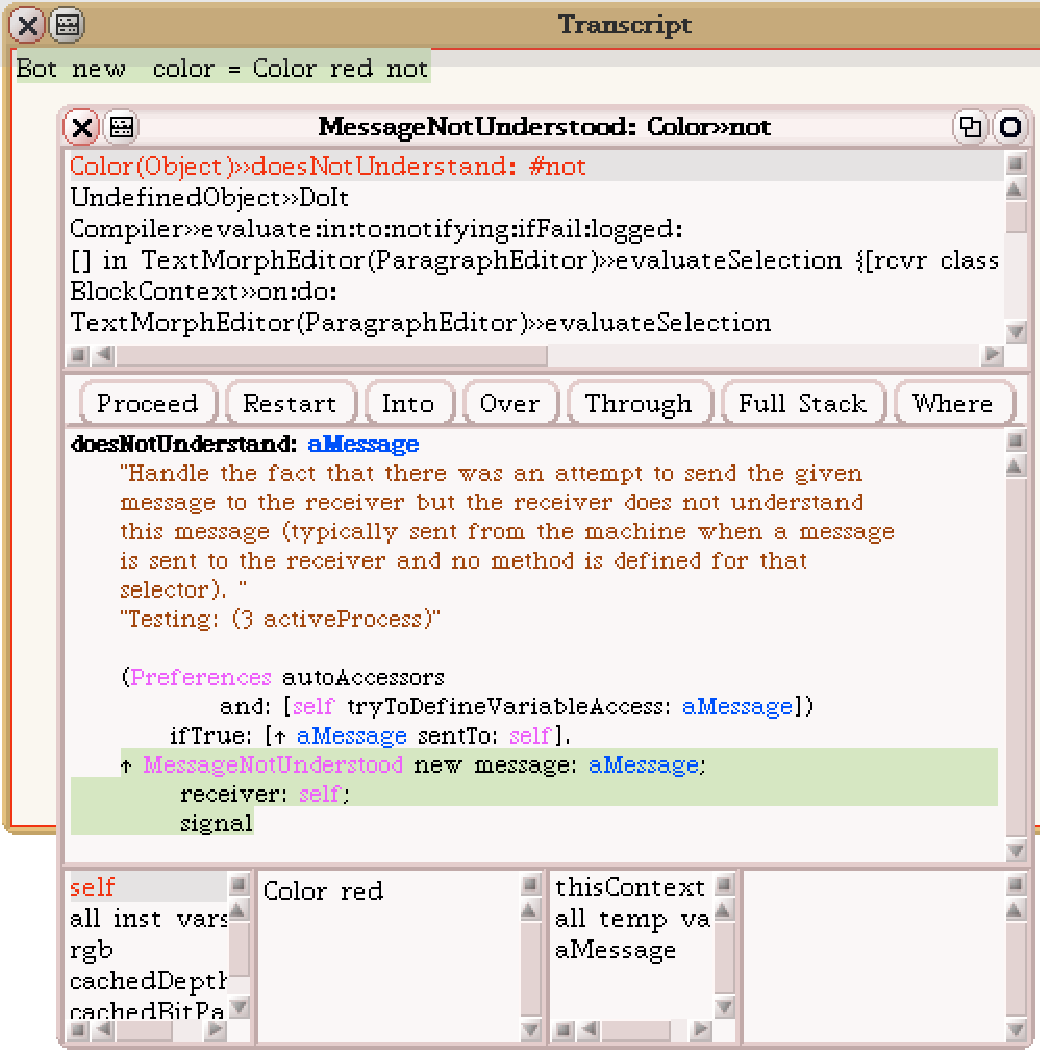
\includegraphics[width=10cm]{colorRedNotDebug}
\caption{The message \ct{not} is not sent to the complete boolean expression \ct{\Turtle new color = Color red}, but sent to the expression \ct{Color red} which returns a color. Therefore it is not understood.\label{fig:wrongnotparenthesis}}
\end{center}
\end{figure}

\paragraph{Using the Debugger.}
The title window of the debugger already gives us some information. \ct{MessageNotUnderstood: Color>>not}. It states that  a color object does not understand the message \ct{not}. 

Now when you select the topmost line of the top pane you see the body of the method \ct{doesNotUnderstand:} which was called as the receiver did not understand the message \ct{not}. When you click on \ct{self} in the left bottom pane, you see that the receiver is not a boolean as it should be but a color \ct{Color red}! If you click on the \ct{aMessage} on the right bottom pane, you will see which message was not understood. In our case, you see \ct{not} which means that the message \ct{not} has not be sent to the right receiver. The message \ct{not} is sent to the result of the expression \ct{Color red} which is a color and does not understand the message \ct{not}. 


\paragraph{Understanding the Problem.}
The reason why the message \ct{not} is sent to the expression \ct{Color red} and not to the complete boolean expression is related to the way \st executes expressions as explained in Chapter~\ref{ch:Evaluating}. First the expressions surrounded by parentheses are executed, then the unary messages, then the binary and finally the keyword-based messages. In our case the message \ct{not} is an unary message. Therefore it is evaluated before the binary message \ct{=} and  it is sent to the result of the expression \ct{Color red}. To get the correct execution order, you have to surround the expression in parentheses as shown in \tscrref{scr:negation}, this way the message \ct{not} will be sent to the result of the \ct{=} message. 

The messages are executed in the wrong expression as follows: The expression \ct{\Turtle new  color = Color red \textbf{not}} is executed as it would be written fully parenthesized as follow \ct{(((\Turtle new) color) = ((Color red) not))}. Therefore first both parts of the binary method \ct{=} are evaluated \ie the expression \ct{((\Turtle new) color)} which returns aColor and the expression
\ct{((Color red) not)}. The execution of the expression \ct{((Color red) not)} evaluates first \ct{Color red} which returns a color, then the message \ct{not} is sent to it which leads to an error.


To get the expected behavior, the expression should be parenthesised so that the \ct{not} message is sent to the result of the \ct{=} message. The expression is then \textbf{(}\Turtle new  color = Color red\textbf{) not}. This expression is executed as follow: first both parts of the binary method \ct{=} are evaluated. Both return a color possibly equal. Then the \ct{=} message is executed, \ie send to the color result of the right hand expression. The execution of the message \ct{=} returns a boolean to which the message \ct{not} is sent. 

When you are not sure about the order of messages, I suggest you use the fact that expressions in parenthesis are executed before the other ones. Therefore you can always put parenthesis around the expressions to make sure that the messages are executed the way you want. 

\subsection*{Similar Problems and Solutions}

It would be tedious to explain the similar problems you may encounter with the other messages such as \ct{\&} and \ct{$\mid$}. Try to execute the scripts \ref{scr:wrongconjunction} and \ref{src:wrongalternative},  and to understand the problems. I show you the corresponding correctly parenthesized scripts~\ref{scr:goodconjunction} and \ref{src:goodalternative}. 

\begin{scriptwithtitle}{Missing Parenthesis to identify the receiver of a \ct{\&}.}\label{scr:wrongconjunction}
| a\Turtle |
a\Turtle := \Turtle new.
a\Turtle center = 100@100 & a\Turtle penSize = 5
\end{scriptwithtitle}

\begin{scriptwithtitle}{Identifying the receiver of a \ct{\&} using parenthesis.}\label{scr:goodconjunction}
| a\Turtle |
a\Turtle := \Turtle new.
\textbf{(}a\Turtle center = 100@100\textbf{)} & \textbf{(}a\Turtle penSize = 5\textbf{)}
\end{scriptwithtitle}


\begin{scriptwithtitle}{Missing Parenthesis to identify the receiver of \ct{$\mid$}.}\label{src:wrongalternative}
| a\Turtle |
a\Turtle := \Turtle new.
a\Turtle center = 100@100 | a\Turtle direction = 90
\end{scriptwithtitle}

\begin{scriptwithtitle}{Identifying the receiver of \ct{$\mid$} using parenthesis.}\label{src:goodalternative}
| a\Turtle |
a\Turtle := \Turtle new.
(a\Turtle center = 100@100) | (a\Turtle direction = 90)
\end{scriptwithtitle}




\summa

\begin{itemize}
\item 
Booleans are \ct{true} or \ct{false}. \ct{true} represents a true fact and \ct{false} a false one.

\item Booleans expressions are expressions that manipulate booleans and that return booleans. 

\item Complex boolean expressions can be composed of simple boolean expressions using conjunction (and), alternation (or), and negation (not). 
\end{itemize}

\begin{center}
\begin{tabular}{| p{2cm}|p{10cm} | p{2cm}|} \hline
  % after \\ : \hline or \cline{col1-col2} \cline{col3-col4} ...
Kind& Message&Results \\ \hline \hline

Negation&\ct{not }&\\ \hline
Examples&\ct{false not}&\ct{true}\\ \hline
&\ct{true not}& \ct{false}\\ \hline
&\ct{(a\Turtle color = Color red) not}&\ct{true} or \ct{false}\\ \hline \hline

Conjunction (and) &\ct{\&}&\\ \hline
Examples&\ct{true \& true}&\ct{true}\\  \hline
&\ct{false \& true}&\ct{false}\\  \hline
&\ct{true \& false}&\ct{false}\\  \hline
&\ct{false \& false}&\ct{false}\\ \hline
&\ct{(a\Turtle center = 100@100) \& (a\Turtle direction = 90)}&\ct{true} or \ct{false}\\ \hline \hline

Alternation (or) &\ct{$\mid$}&\\ \hline
Examples&\ct{true $\mid$ true}&\ct{true}\\ \hline
&\ct{false $\mid$ true}&\ct{true}\\\hline
&\ct{true $\mid$ false}&\ct{true}\\ \hline
&\ct{false $\mid$ false}&\ct{false}\\ \hline
&\ct{Time now > (Time new hours: 8) $\mid$  (Date today  weekday asString = 'Sunday')}&\ct{true} or \ct{false}\\ \hline \hline
\end{tabular}
\end{center}


\ifx\wholebook\relax\else\end{document}\fi





